\documentclass[border=2pt]{standalone}
\usepackage[T1]{fontenc}
\usepackage[utf8]{inputenc}
\usepackage{mathptmx}
\usepackage{tikz}
\usetikzlibrary{arrows.meta,calc}
\begin{document}
\begin{tikzpicture}[x=9cm,y=7.509cm,
  lab/.style={font=\footnotesize,align=center},
  seta/.style={-{Stealth[length=2.2mm]},white,line width=0.9pt},
  borda/.style={-{Stealth[length=2.2mm]},black,line width=0.6pt}]
  \node[anchor=south west,inner sep=0] at (0,0) {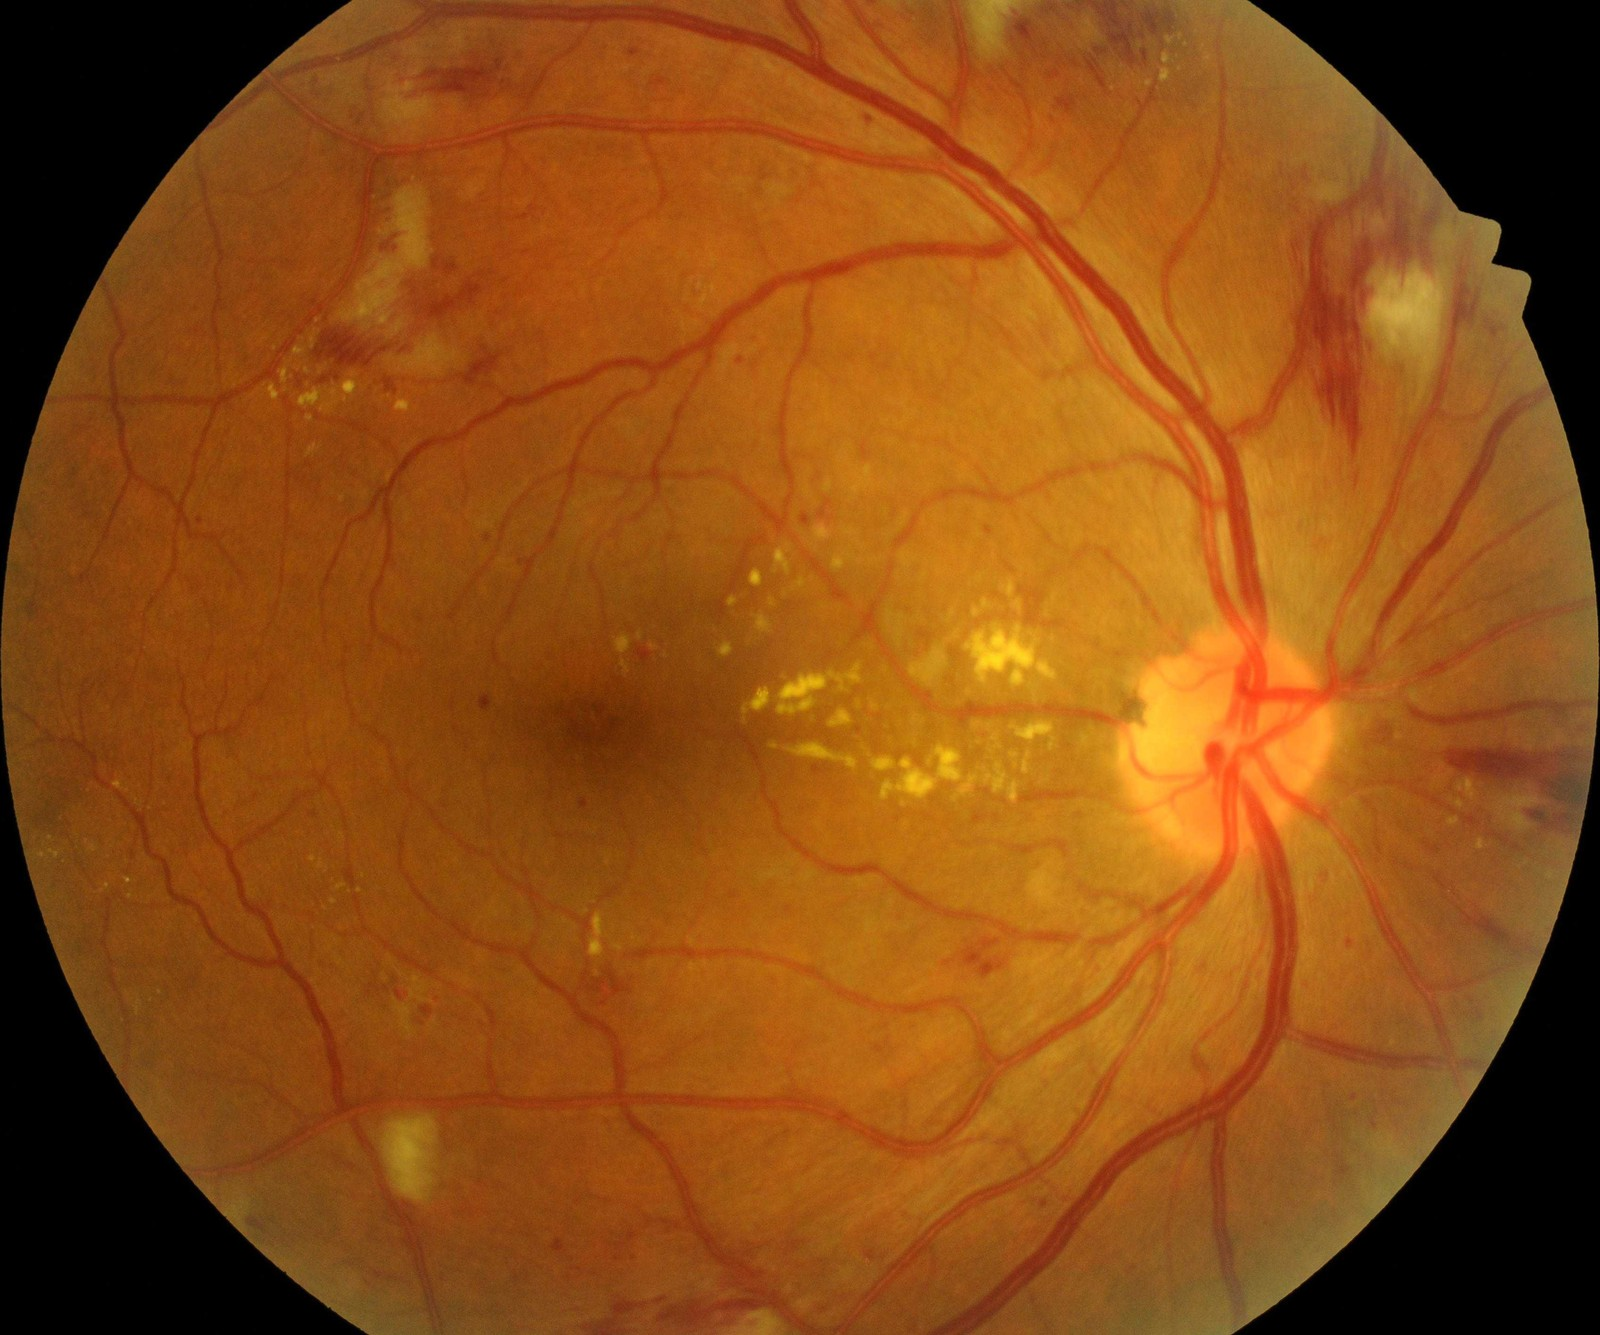
\includegraphics[width=9cm]{../fig-idrid22.jpg}};
  % coordenadas normalizadas (x da esquerda, y de baixo)
  \coordinate (se1) at (0.245,0.810);
  \coordinate (se2) at (0.880,0.753);
  \coordinate (se3) at (0.249,0.130);
  \coordinate (ex)  at (0.566,0.480);
  \coordinate (od)  at (0.763,0.443);
  \coordinate (fov) at (0.364,0.466);
  % rótulos fora da imagem, setas contínuas com contorno preto
  \newcommand{\seta}[2]{\draw[-{Stealth[length=2.6mm]},black,line width=2.0pt] #1 -- #2;
    \draw[-{Stealth[length=2.0mm]},white,line width=0.9pt,shorten >=0.4pt] #1 -- #2;}
  \node[lab,anchor=east] (lse) at (-0.03,0.80) {Mancha algodonosa\\(exsudato mole)};
  \node[lab,anchor=east] (lfov) at (-0.03,0.47) {Fóvea};
  \node[lab,anchor=west] (lse2) at (1.03,0.80) {Mancha\\algodonosa};
  \node[lab,anchor=west] (lod) at (1.03,0.44) {Disco óptico};
  \node[lab,anchor=west] (lex) at (1.03,0.18) {Exsudatos duros};
  \seta{(lse.east)}{($(se1)+(-0.035,0)$)}
  \node[lab,anchor=east] (lse3) at (-0.03,0.13) {Mancha\\algodonosa};
  \seta{(lse3.east)}{($(se3)+(-0.04,0)$)}
  \seta{(lfov.east)}{($(fov)+(-0.035,0)$)}
  \seta{(lse2.west)}{($(se2)+(0.04,0.01)$)}
  \seta{(lod.west)}{($(od)+(0.06,0)$)}
  \seta{(lex.west)}{($(ex)+(0.01,-0.05)$)}
\end{tikzpicture}
\end{document}
